\begin{frame}{Air Time of a LoRa Frame and the Duty Cycle}
  \only<1>{
    One can calculate the air time by hand \ldots
    \begin{center}
      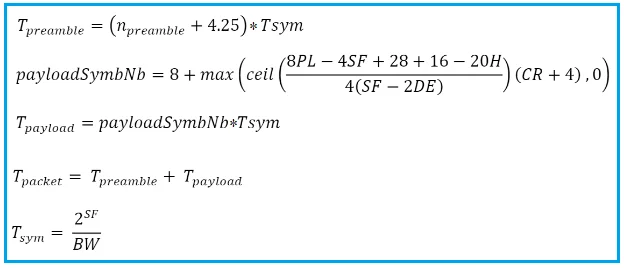
\includegraphics[width=0.7\textwidth]{material/LoRaWAN-packet-duration-calculation-formula.png}
    \end{center}
  }
  \only<2>{
    \ldots but it's much easier to use an online air time calculator:
    \vskip1em
    \begin{columns}[onlytextwidth]
      \begin{column}{0.45\textwidth}
        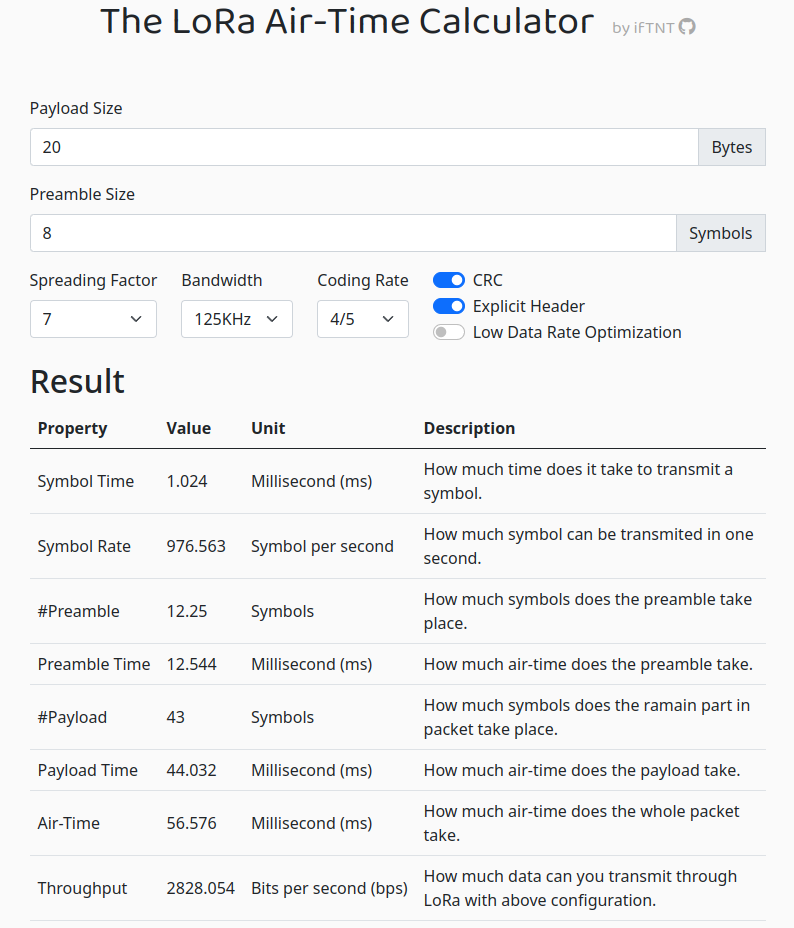
\includegraphics[width=0.85\textwidth]{material/lora-airtime-calculator.png}
      \end{column}
      \begin{column}{0.55\textwidth}.
        \begin{exampleblock}{The Duty Cycle $D$}
          Example: A LoRa device transmits 20 payload bytes ($SF=7,\,BW=\SI{125}{\kilo\hertz}\,CR=1\,(4/5),$) every minute.
          \begin{itemize}
            \item The \alert{air} (duty) time is $t_a = \SI{56.576}{\milli\second}$.
            \item The \alert{cycle} time is $t_c = \SI{60}{\second} = \SI{60000}{\milli\second}$.
            \begin{description}[$\Rightarrow$]
              \item[$\Rightarrow$] The \alert{duty cycle $D$} is the \alert{fraction} of used \alert{air} time per \alert{cycle} time \alert{in percent}. $$D = \frac{t_a}{t_c}\cdot 100 = \frac{\SI{56.576}{}}{\SI{60000}{}}\cdot 100 = \SI{0,09}{\percent}$$
            \end{description}
          \end{itemize}
        \end{exampleblock}
      \end{column}
    \end{columns}
  }
\end{frame}
